\documentclass[12pt,a4paper]{article}

\usepackage[utf8]{inputenc}
\usepackage[T2A]{fontenc}
\usepackage[ukrainian]{babel}

\usepackage{geometry}
\geometry{left=2cm,right=2cm,top=2cm,bottom=2cm}

\usepackage{graphicx}
\usepackage{array,multirow}
\usepackage{booktabs}
\usepackage{caption}
\usepackage{subcaption}
\renewcommand{\thetable}{№\arabic{table}}

\usepackage{amsmath}
\usepackage{pdflscape}
\usepackage{xcolor}

\usepackage{hyperref}

\renewcommand\thesubfigure{(\alph{subfigure})}

\begin{document}

    \begin{titlepage}

        % Картинка шапки (по центру, з відступом від верху)
        \begin{center}
\includegraphics[width=0.7\textwidth]{../../../TITLES/letterhead.png}\end{center}

        \begin{center}
            \large Національний технічний університет України\\
            «Київський політехнічний інститут імені Ігоря Сікорського»\\[1em]
            Факультет інформатики та обчислювальної техніки\\
            Кафедра обчислювальної техніки
        \end{center}

        \vfill

        \begin{center}
            \textbf{\LARGE Практична електроніка}\\[2em]
            \textbf{\Large Лабораторна робота №6}\\[1em]
            «Дослідження цифро-аналогових перетворювачів»
        \end{center}

        \vfill

        \begin{flushright}
            Виконав: студент 2 курсу ФІОТ, гр. ІО-41\\
            \textit{Давидчук А.~М.}\\[1em]
            Перевірив: \textit{Гайдай А.~Р.}
        \end{flushright}

        \vfill

        \begin{center}Київ --- 2025\end{center}

    \end{titlepage}

    % Основний документ:

    \setlength{\parindent}{0em}

    \textbf{\underline{Тема:}} «Дослідження імпульсних тригерів, аналогових компараторів та схем формування рівнів».

    \vspace{1em}

    \textbf{\underline{Мета:}} Дослідити принцип дії, основні властивості та характеристики цифроаналогових перетворювачів (ЦАП). Ознайомитись із основними видами,
параметрами цих пристроїв та областю їх застосування.

    \begin{center} \textbf{\Large Практична частина} \end{center}

    Мій номер залікової книги 6, звідси $N = 6$.

    \begin{center} \textbf{\large Аналіз схеми №1: ЦАП із підсумовуванням напруг} \end{center}

    \setlength{\parindent}{1.5em}

    Нижче наведено приклад схеми ЦАП із підсумовуванням напруг, яку зібрано
    у середовищі MicroCap:

    \begin{figure}[h!]

        \renewcommand{\thefigure}{\arabic{figure}} % робимо "3.1", "3.2" і т.д.

        \centering
        \includegraphics[width=0.7\textwidth]{scheme1.pdf}
        \caption{Схема ЦАП із підсумовуванням напруг}

    \end{figure}

    Нижче наведено часові діаграми роботи (рис.~2) схеми, яку наведено на рис.~1.
    На рис.~2 зображено зміни у часі суми напруг \(U_{\text{sum}}\) та вихідної
    напруги \(U_{\text{out}}\) ЦАП із підсумовуванням напруг у залежності від
    комбінацій розрядів \(a_0\ldots a_2\). Сигнали на розрядах задаються
    послідовністю прямокутних імпульсів. Частота меншого розряду у двічі
    більша, ніж частота наступного. Даний ЦАП реалізує формулу

    \begin{equation}
    U_{\text{вих}} = 
    \frac{U_{\text{оп}}}{2^{n}}
    \sum_{i=0}^{n-1} a_i \cdot 2^{i}.
    \end{equation}

    де
    \(U_{\text{оп}}=8~\text{В}\), \(n=3\). Коефіцієнт підсилення
    коопераційного підсилювача, на неінвертувальний вхід якого надходить
    сума напруг \(U_{\text{sum}}\), дорівнює:
    \[
    \left(\frac{R_7}{R_8}+1\right)=\frac{1\,\text{k}\Omega}{1\,\text{k}\Omega}+1=2.
    \]

    \newpage

    \begin{figure}[h!]
        \centering
        
\includegraphics[width=\linewidth]{graph1.png}
        \caption{\centering Часові діаграми роботи схеми, яку наведено на рис. 1. 
}
    \end{figure}

    Максимальна вихідна напруга:
    \[
    U_{\text{вих max}} = 2 \cdot 8 = 16 = U_{\text{оп}} 
    \left( \frac{1}{2} + \frac{1}{4} + \frac{1}{8} + \ldots + \frac{1}{2^n} \right)
    = k \cdot \frac{U_{\text{оп}}}{2^n} \sum_{i=0}^{n-1} 2^i
    \]

    а максимальна сумарна напруга на вході ІМС ОП:
    \[
    U_{\text{sum.max}} = \frac{U_{\text{оп}}}{2^n} \sum_{i=0}^{n-1} 2^i 
    = 8 \cdot \frac{7}{8} = 7
    \]

    Коефіцієнт передачі (розмір кроку квантування за рівнем), тобто розрахункове
    збільшення вихідної напруги під час зміни вхідного коду на одиницю молодшого
    розряду (ціна молодшого значущого розряду — МЗР), складає:
    \[
    K_{\text{ЦАП}} = \frac{U_{\text{оп}}}{2^n} = \frac{8}{8} = 1 
    \left[ \frac{\text{В}}{\text{МЗР}} \right]
    \]

    Для прикладу розрахунку візьмемо ДВК: 
    \[
    100_{(2)} = 4_{(10)}.
    \]

    \[
    U_{\text{SUM}} = 4 \cdot 1 = 4~\text{В},
    \qquad
    U_{\text{ВИХ}} = 4 \cdot 2 = 8~\text{В}.
    \]

    На рис.~2 видно, що теоретичні розрахунки збігаються з експериментальними даними.

    \newpage

    \begin{center} \textbf{\large Аналіз схеми №2: ЦАП із підсумовуванням струмів} \end{center}

    Нижче наведено приклад схеми ЦАП із підсумовуванням струмів, яку зібрано
у середовищі MicroCap:

    \begin{figure}[h!]

        \renewcommand{\thefigure}{\arabic{figure}} % робимо "3.1", "3.2" і т.д.

        \centering
        \includegraphics[width=0.7\textwidth]{scheme2.pdf}
        \caption{Схема ЦАП із підсумовуванням струмів}

    \end{figure}

    На рис. 4 зображено часові діаграми роботи схеми, яку наведено на рис. 3, в залежності від комбінацій розрядів $a_0 \dots a_3$.

    Сигнали на відповідних розрядах задаються послідовністю прямокутних
    імпульсів. Частота меншого розряду є вдвічі більшою, ніж частота наступного:

    \begin{figure}[h!]
        \centering
        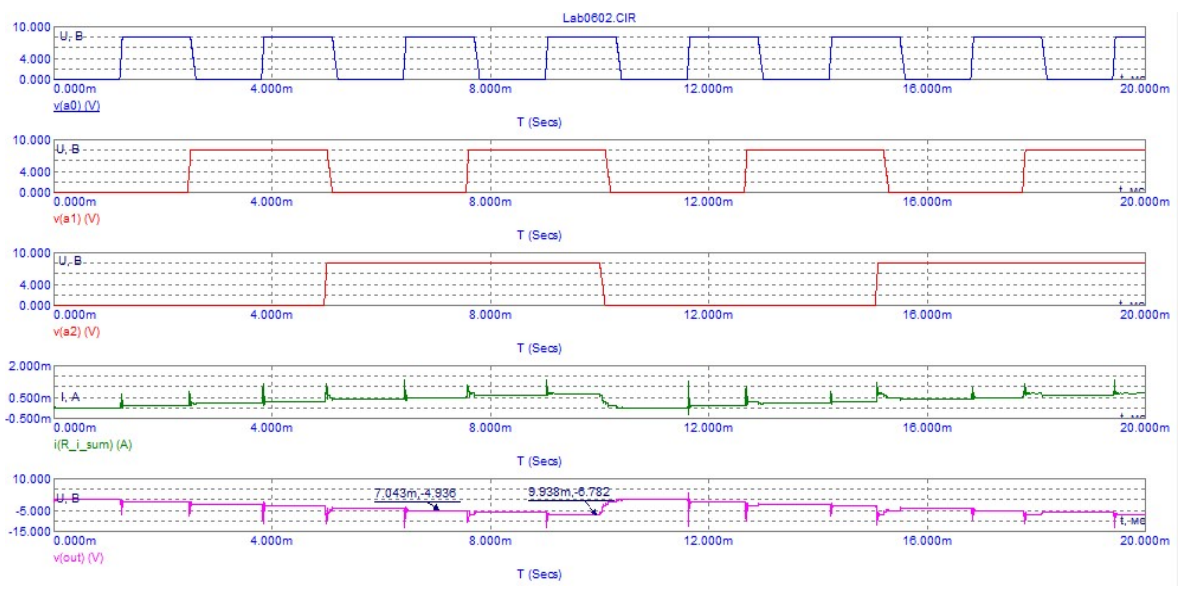
\includegraphics[width=\linewidth]{graph2_.png}
        \caption{\centering Часові діаграми роботи схеми, яку наведено на рис. 3}
    \end{figure}

    \newpage

    Якщо число розрядів вхідного двійкового коду дорівнює $n$, то
    \[
    \displaystyle U_{\text{вих,max}} = -\Bigl(1-2^{-n}\Bigr)\!\left(\frac{U_{\text{оп}}\cdot R_{33}}{R}\right).
    \]

    Якщо число розрядів вхідного двійкового коду дорівнює: $n=3$, $R_{33}=R=10\text{ k}\Omega$, $U_{\text{оп}}=8$, то
    \[
    \displaystyle
    U_{\text{вих,max}}
    = -\,U_{\text{оп}}\frac{R_{33}}{R}\!\left(\frac12 + \frac14 + \cdots + \frac{1}{2^{n}}\right)
    = -\,U_{\text{оп}}\frac{R_{33}}{R}\cdot \frac12\sum_{i=0}^{n-1}2^{-i} =
    \]
    \[
    = -\,U_{\text{оп}}\frac{R_{33}}{R}\Bigl(1-2^{-n}\Bigr)
    = -\,8\cdot\frac{10\text{ k}\Omega}{10\text{ k}\Omega}\cdot\frac{7}{8}
    = -7~\text{В}.
    \]

    Коефіцієнт передачі (розмір кроку квантування за рівнем), тобто розрахункове збільшення вихідної напруги під час зміни вхідного коду на одиницю молодшого розряду (ціна молодшого значущого розряду, МЗР), складає:
    \[
    \displaystyle
    K_{\text{ЦАП}}
    = \frac{\Delta U_{\text{вих}}}{1~\text{МЗР}}
    = -\,\frac{U_{\text{оп}}\,R_{33}}{R\cdot 2^{n}}
    = -\,\frac{8\cdot 10}{10\cdot 8}
    = -1\ \left[\frac{\text{В}}{\text{МЗР}}\right].
    \]

    Для прикладу розрахунку візьмемо ДК $\,101_{(2)}=5_{(10)}$. Звіримо теоретичні розрахунки з експериментальними даними:
    \[
    \displaystyle
    U_{\text{вих}}
    = -\,U_{\text{оп}}\frac{R_{33}}{R}\!\left(\frac12 + 0 + \frac18\right)
    = -\,8\cdot\frac{10\text{ k}\Omega}{10\text{ k}\Omega}\cdot\frac{5}{8}
    = -5~\text{В}.
    \]

    На рис.~4 бачимо, що теоретичні розрахунки збігаються з експериментальними даними.

    \vspace{1em}

    \noindent
    \textbf{\underline{Висновок:}}
    У ході виконання лабораторної роботи було досліджено принцип дії, основні властивості та характеристики цифро-аналогових перетворювачів (ЦАП).  
    Було розглянуто два типи схем: ЦАП із підсумовуванням напруг та ЦАП із підсумовуванням струмів.

    Для кожної схеми виконано теоретичні розрахунки та проведено моделювання у середовищі \texttt{MicroCap}.  
    Отримано часові діаграми вихідних сигналів, що підтвердили правильність роботи схем і збіг теоретичних та експериментальних результатів.

    Під час дослідження визначено:
    \begin{itemize}
    \item залежність вихідної напруги від вхідного двійкового коду;
    \item максимальну вихідну напругу $U_{\text{вих,max}}$ для різних значень $n$;
    \item коефіцієнт передачі (розмір кроку квантування) $K_{\text{ЦАП}}$, який визначає зміну вихідної напруги при зміні молодшого розряду коду;
    \item практичне підтвердження формули $U_{\text{вих}} = f(a_0, a_1, a_2, \ldots, a_n)$.
    \end{itemize}

    У результаті експерименту встановлено, що значення вихідної напруги, отримані під час моделювання, повністю збігаються з розрахунковими.  
    Таким чином, підтверджено справедливість теоретичних співвідношень та правильність побудови схем цифро-аналогов- их перетворювачів.  
    Отримані знання дозволяють краще зрозуміти принцип роботи ЦАП і його застосування в цифрових системах керування та вимірювання.

\end{document}